\section{Method}
The experimental setup consisted of an X-ray source pointing on a sample of powdered crystal. The sample was placed on a diffractometer connected to a computer to control the placement of the sample. Behind the sample was a large area detector used to capture the diffraction rings. The setup can bee seen in \ref{fig:setup}
\begin{figure}[H]
    \centering
    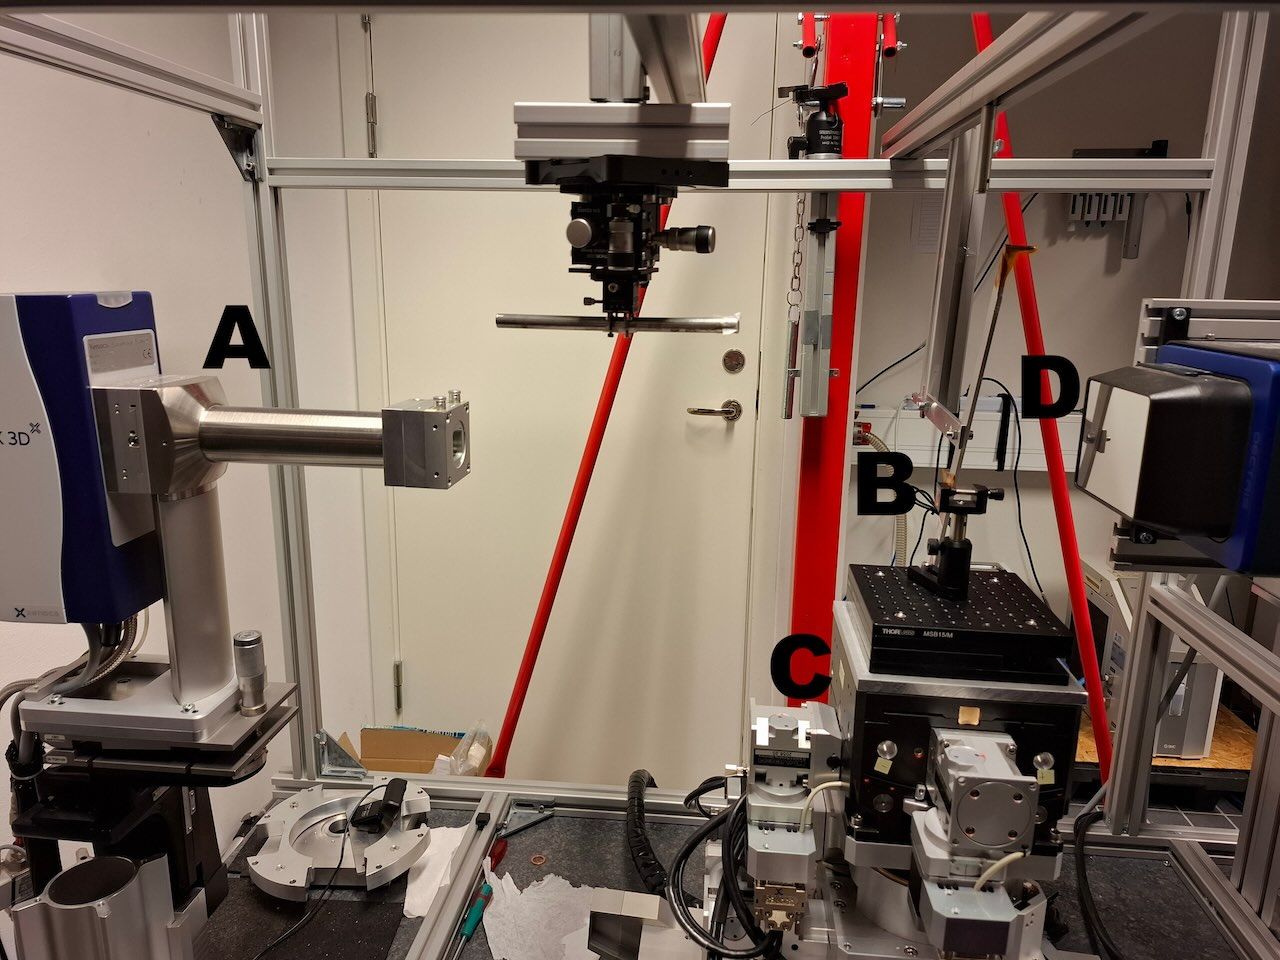
\includegraphics[width=0.7\textwidth]{Figures/setup_letters.jpg}
    \caption{The experimental setup. \textbf{A} ist he X-ray source, \textbf{B} is the sample, \textbf{C} is the diffractometer and \textbf{D} is the detector.}
    \label{fig:setup}
\end{figure}


The energy of the x-rays are \SI{17.45}{\kilo\electronvolt}. 

The detector uses six semiconductors. 

Calibrations of hex.., this is good since we have a lot of diffraction rings.  

1. Put in all the data
2. mask out dead spots
3. Tell where the rings are 
4. The image is converted to an intensity plot (Note that the x-axis is in $2\theta$). 


Hot pixel, high peak with no width. The pixel can be burnt out. 
